
\documentclass[./Thick_TQFTs_and_Quantum_Information.tex]{subfiles}

\begin{document}

\section{Category of Connections}

We now make precise the notion of a category of ``parallel transport machinery''
as mentioned in the previous section. For a vector bundle $\pi_E : E \to M$, we
write $\Gamma(E)$ to denote the set\footnote{We are not using any sheaf theory,
yet.} of sections of the bundle. We recall that a connection on $E$ is a
function
\[
  \nabla : \Gamma(TM \tensor E) \to \Gamma(E)
\]
satisfying some algebraic properties that are not important at the moment.
Suppose we have another bundle $\pi_{E'} : E \to M$ with a bundle morphism
$f = (u, v) : E \to E'$ -- a pair of maps $u : M \to M'$ and $v : E \to E'$
with $v$ linear on each fibres of $E$, making the following diagram commute:
\[\begin{tikzpicture}[baseline=(a).base]
\node[scale=\diagscale] (a) at (0, 0){
\begin{tikzcd}
E \ar[d, "\pi_E" left] \ar[r, "v" above] & E' \ar[d, "\pi_{E'}" right]\\
M \ar[r, "u" below] & M'
\end{tikzcd}
};
\end{tikzpicture}\]
The derivative of $u$ induces a bundle morphism
$(du \tensor v, u) : TM \tensor E \to TM' \tensor E'$, where
$(du \tensor v)(x \tensor y) = du(x) \tensor v(x)$ for $x \in TM$ and
$y \in E$. If, in addition, $f$ has an inverse $f^{-1} = (u^{-1}, v^{-1})$,
we have an induced mapping
$\wh{f} : \Gamma(TM' \tensor E') \to \Gamma(TM \tensor E)$ given, for each $s
\in \Gamma(TM' \tensor E')$, by the composite:
\[\begin{tikzpicture}[baseline=(a).base]
\node[scale=\diagscale] (a) at (0, 0){
\begin{tikzcd}[column sep=55, row sep=large]
TM \tensor E &
TM' \tensor E' \ar[l, "d(u^{-1}) \tensor v^{-1}" above]\\
M \ar[u, "\wh{f}(s)" left] \ar[r, "u" below]
& M' \ar[u, "s" right]
\end{tikzcd}
};
\end{tikzpicture}\]
Note that $d(u^{-1}) = (du)^{-1}$ so we will unambiguously write $du^{-1}$ from
this point. Now, $\nabla(\wh{f}(s))$ is a section of $E$ while
$(f \odot \nabla)(s) := v\nabla(\wh{f}(s))u^{-1}$ is a section of $E'$:
\[\begin{tikzpicture}[baseline=(a).base]
\node[scale=\diagscale] (a) at (0, 0){
\begin{tikzcd}[column sep=large, row sep=large]
E \ar[r, "v" above] &
E'\\
M \ar[u, "\nabla(\wh{f}(s))" left] &
M' \ar[u, "(f \odot \nabla)(s)" right] \ar[l, "u^{-1}" below]
\end{tikzcd}
};
\end{tikzpicture}\]
This yields a function:
\[\begin{array}{ccccl}
f \odot \nabla
&:& \Gamma(TM' \tensor E') &\to& \Gamma(E) \\
&:& X \tensor s &\mapsto&
    v\nabla((du^{-1} \tensor v^{-1})(X \tensor s)u)u^{-1} \\
& &             & = & v\nabla(du^{-1}Xu \tensor v^{-1}su)u^{-1}
\end{array}\]
In the last equality, we used the fact that
\[
  (X \tensor s)u = Xu \tensor su
\]
which follows from the definition of the tensor product of bundles. Using this
construction, we will define our desired double category.

\subsection{Bundle Isomorphisms Transform Connections}

We wish to show that $f \odot \nabla$ is a connection. For this, we recall the
properties of a connection. Let $\pi_E : E \to M$ be a vector bundle as before
with $X, Y \in \Gamma(TM)$, $s, t \in \Gamma(E)$, $r \in C^{\infty}(M, \R)$.
Then, $\nabla : \Gamma(TM \tensor E) \to \Gamma(E)$ is a conneciton if and only
if the following hold:
\[\begin{array}{lll}
\nabla((X + Y) \tensor s) &= \nabla(X \tensor s) + \nabla(Y \tensor s)
  & (\text{Additivity in $\Gamma(TM)$}) \\
\nabla(X \tensor (s + t)) &= \nabla(X \tensor s) + \nabla(X \tensor t)
  & (\text{Additivity in $\Gamma(E)$}) \\
\nabla((r \cdot X) \tensor s) &= r \cdot \nabla(X \tensor s)
  & (\text{Scalar-multiplicativity in $\Gamma(TM)$}) \\
\nabla(X \tensor (r \cdot s)) &= dr(X) \cdot s + r \cdot \nabla(X \tensor s)
  & (\text{Leibniz property in $\Gamma(E)$}) \\
\end{array}\]
\begin{rmk}
The map $dr(X)$ in the Leibniz property is defined as follows. If $r : M \to \R$
is a smooth function, then we have $dr : TM \to T\R$, where
$\pi_{T\R} : T\R \to \R$ is the tangent bundle on $\R$. Given a section
$X : M \to TM$, we obtain a smooth map $drX : M \to T\R$. As a result, $drX$
yields a smooth map $dr(X) := \pi_{T\R}drX : M \to \R$. That is, the derivative
$dr$ yields a map
\[
  dr : \Gamma(TM) \to C^{\infty}(M, \R)
\]
which is the one in Leibniz property above.
\end{rmk}

Now, let $X, Y \in \Gamma(TM')$, $s \in \Gamma(E')$, $r \in C^{\infty}(M', \R)$.
We recall some basic identities that will be of use in showing that
$f \odot \nabla$ is a connection:
\begin{align*}
(X + Y)u &= Xu + Yu && \text{by definition of pointwise addition} \\
(r \cdot X)u &= (ru) \cdot Xu && \text{by definition of pointwise scaling} \\
v(X + Y) &= vX + vY && \text{fibre-wise linearity of $v$} \\
v(r \cdot X) &= r \cdot vX && \text{fibre-wise linearity of $v$}
\end{align*}
We note that these identities hold for arbitrary bundle morphisms $(u, v)$,
smooth real-valued maps $r$ and sections $X, Y$, as long as the operations are
well-defined.

We now proceed to check that $f \odot \nabla$ is a connection. To this end, we
first check additivity in the $\Gamma(TM')$ coordinate.
\begin{align*}
(f \odot \nabla)((X + Y) \tensor s)
=& v\nabla(du^{-1}(X + Y)u \tensor v^{-1}su)u^{-1} \\
=& v\nabla((du^{-1}Xu + du^{-1}Yu) \tensor v^{-1}su)u^{-1} \\
=& v(\nabla(du^{-1}Xu \tensor v^{-1}su)
 + \nabla(du^{-1}Yu \tensor v^{-1}su))u^{-1} \\
=& v\nabla(du^{-1}Xu \tensor v^{-1}su)u^{-1}
 + v\nabla(du^{-1}Yu \tensor v^{-1}su))u^{-1} \\
=& (f \odot \nabla)(X \tensor s) + (f \odot \nabla)(Y \tensor s)
\end{align*}
Additivity in the $\Gamma(E')$ coordinate is similar. So, we check scalar
multiplicativity in the $\Gamma(TM')$ coordinate:
\begin{align*}
(f \odot \nabla)(r \cdot X \tensor s)
=& v\nabla(du^{-1}(r \cdot X)u \tensor v^{-1}su)u^{-1} \\
=& v\nabla(du^{-1}(ru \cdot Xu) \tensor v^{-1}su)u^{-1} \\
=& v\nabla((ru \cdot (du^{-1}Xu)) \tensor v^{-1}su)u^{-1} \\
=& v (ru \cdot \nabla(du^{-1}Xu \tensor v^{-1}su))u^{-1} \\
=& v (ruu^{-1} \cdot \nabla(du^{-1}Xu \tensor v^{-1}su)u^{-1}) \\
=& r \cdot (v\nabla(du^{-1}Xu \tensor v^{-1}su)u^{-1}) \\
=& r \cdot ((f \odot \nabla)(X \tensor s))
\end{align*}

We finally check the Liebnitz rule.
\begin{align*}
(f \odot \nabla)(X \tensor (r \cdot s))
=& v\nabla(du^{-1}Xu \tensor v^{-1}(r \cdot s)u)u^{-1} \\
=& v(\nabla(du^{-1}Xu \tensor v^{-1}(ru \cdot su))u^{-1} \\
=& v\nabla(du^{-1}Xu \tensor ru \cdot (v^{-1}su))u^{-1} \\
=& v(
      d(ru)(du^{-1}Xu) \cdot v^{-1}su
      + ru \cdot \nabla(du^{-1}Xu \tensor v^{-1}su)
    )u^{-1} \\
=& v(d(ru)(du^{-1}Xu) \cdot v^{-1}su)u^{-1}
 + v(ru \cdot \nabla(du^{-1}Xu \tensor v^{-1}su))u^{-1}
\end{align*}
It now suffices to show that the left summand is
\[
  dr(X) \cdot s
\]
and the right summand is
\[
  r \cdot (f \odot \nabla)(X \tensor s)
\]
For the right summand, we observe:
\begin{align*}
 & v(ru \cdot \nabla(du^{-1}Xu \tensor v^{-1}su))u^{-1} \\
=& v(ruu^{-1} \cdot \nabla(du^{-1}Xu \tensor v^{-1}su)u^{-1}) \\
=& v(r \cdot \nabla(du^{-1}Xu \tensor v^{-1}su)u^{-1}) \\
=&r \cdot (v\nabla(du^{-1}Xu \tensor v^{-1}su)u^{-1}) \\
=& r \cdot (f \odot \nabla)(X \tensor s)
\end{align*}
For the left summand, we first observe a useful property of the derivative
operator $d-$. If $g : L \to M$ and $h : M \to N$ are smooth maps, then by the
pasting of pushout diagrams to give pushout diagrams, we have
\[
  d(h \circ g) = dh \circ dg
\]
Then, we have:
\begin{align*}
v(d(ru)(du^{-1}Xu) \cdot v^{-1}su)u^{-1}
=& v(\pi_{T\R}d(ru)(du^{-1}Xu) \cdot v^{-1}su)u^{-1}\\
=& v(\pi_{T\R}d(ruu^{-1})Xu \cdot v^{-1}su)u^{-1}\\
=& v(\pi_{T\R}drXu \cdot v^{-1}su)u^{-1}\\
=& v((\pi_{T\R}drX \cdot v^{-1}s)u)u^{-1}\\
=& v(v^{-1}(\pi_{T\R}drX \cdot s)u)u^{-1}\\
=& dr(X) \cdot s
\end{align*}
as required. This completes the proof of the following theorem.
\begin{thm}
Let $\pi : E \to M$, $\pi' : E' \to M'$ be bundles with a bundle isomorphism
$f = (u, v) : E \to E'$. If $\nabla$ is a connection on $\pi$, then
$f \odot \nabla$ is a connection on $\pi'$.
\end{thm}
\begin{defn}
We call $f \odot \nabla$ the shift of $\nabla$ along $f$ and say that $f$
takes $\nabla$ to $f \odot \nabla$. From this point, we write $f\nabla$ as
opposed to $f \odot \nabla$, whenever there is no confusion.
\end{defn}

\subsection{Category of Connections}

Let $\pi_i : E_i \to M_i$ be a bundles equipped with a connections $\nabla_i$
for $i \in \set{1, 2, 3, 4}$. Let $f_{i, i + 1} = (u_{i, i + 1}, v_{i, i + 1})$
be bundle isomorphisms for $i \in \set{1, 2, 3}$. Then, the composite
$f_{1, 3} := f_{2, 3}f_{1, 2} = (u_{2, 3}u_{1, 2}, v_{2, 3}v_{1, 2})
=: (u_{1, 3}, v_{1, 3})$ is clearly a bundle isomorphism. We similarly define
composites $f_{i, j}$ for each $i < j \in \set{1, 2, 3, 4}$. Now, suppose
$\nabla_{i + 1} = f_{i, i + 1}\nabla_i$ for each $i \in \set{1, 2, 3}$. Then, we
immediately have
\[
  f_{i, k}\nabla_i = f_{j, k}f_{i, j}\nabla_i = f_{j, k}\nabla_j = \nabla_k
\]
for each $i < j < k$ in $\set{1, 2, 3, 4}$. In particular,
\[
  f_{3, 4}(f_{2, 3}f_{1, 2}\nabla_1) = \nabla_4
    = (f_{3, 4}f_{2, 3})f_{1, 2}\nabla_1
\]

We then observe the action of identity bundle morphisms. The identity bundle
morphism on $\pi_1$ is the pair $\id_{\pi_1} = (\id_{E_1}, \id_{M_1})$. Then,
\begin{align*}
   \id_{\pi_1}\nabla_1(X \tensor s)
&= \id_{E_1}\nabla_1(d(\id_{M_1})^{-1}X\id_{M_1}
                     \tensor \id_{E_1}^{-1}s\id_{M_1})\id_{M_1}^{-1} \\
&= \nabla_1(\id_{TM_1}^{-1}X \tensor s) \\
&= \nabla_1(X \tensor s)
\end{align*}
so that $\id_{\pi_1}\nabla = \nabla$. We finally observe that
$ff^{-1}\nabla = \id\nabla = \nabla$ for any connection $\nabla$ and any
compatible diffeomorphism $f$.

These observations motivate the following definition.
\begin{defn}
Let $\pi_1$ and $\pi_2$ be bundles equipped with connections $\nabla_1$ and
$\nabla_2$ respectively. Then, a bundle isomorphism
$f = (u, v) : \pi_1 \to \pi_2$ satisfying $f\nabla_1 = \nabla_2$ is called an
isomorphism, or simply morphism, of connections.
\end{defn}

From the work above, we have established the following results.
\begin{thm}
There exists a groupoid, denoted $\Conn$, whose objects are connections and
whose morphisms are isomorphisms of connections.
\end{thm}
\begin{defn}[Category of Connections]
We will call the category of the above function the category or groupoid of
connections. We will denote this category $\Conn$.
\end{defn}

We now try to establish a monoidal structure for a subcategory of the category
of connections. Let $\nabla_1$ and $\nabla_2$ be two connections with underlying
bundles $\pi_1 : E_1 \to M_1$ and $\pi_2 : E_2 \to M_2$ respectively. We will
consider the coproduct or disjoint union of these bundles in the category of
manifolds. There exists a smooth map
$\pi_1 \amalg \pi_2 : E_1 \amalg E_2 \to M_1 \amalg M_2$ which we will give the
structure of a vector bundle as follows. For this, we additionally assume that
the fibres of $E_1$ and $E_2$ are the same vector space. Let
$U = U_1 \amalg U_2, V = V_1 \amalg V_2$ be open sets in $M_1 \amalg M_2$ with
$U_i, V_i \subset M_i$ for $i \in \set{1, 2}$, and consider
$(U_1 \amalg U_2) \cap (V_1 \amalg V_2) = (U_1 \cap V_1) \amalg (U_2 \cap V_2)$.
We have a transition function $G_{U_1, V_1}$ on $U_1 \cap V_1$ from the bundle
$\pi_1$ and one $H_{U_2, V_2}$ on $U_2 \cap V_2$ from $\pi_2$. We define a
function $(G \amalg H)_{U, V} : U \cap V \to \GL_n(\C)$ piecewise, as
follows:
\[
  (G \amalg H)_{U, V}(x) := \begin{cases}
    G_{U_1, V_1}(x), & x \in U_1 \cap V_1 \subset M_1 \\
    H_{U_2, V_2}(x), & x \in U_2 \cap V_2 \subset M_2
  \end{cases}
\]
which is smooth since it is a disjoint union of smooth functions. Therefore,
\[
  G \amalg H := \set[(G \amalg H)_{U, V}]
                    {U, V \subset M_1 \amalg M_2 \text{ are open}}
\]
is a vector bundle structure on $\pi_1 \amalg \pi_2$. A section of
$E_1 \amalg E_2$ is a smooth map
\[
  s : M_1 \amalg M_2 \to E_1 \amalg E_2
\]
satisfying $(\pi_1 \amalg \pi_2)s = \id_{M_1 \amalg M_2}$. We note that this
guarantees that the $s = s_1 \amalg s_2$ where $s_i$ is a section of
$E_i$, $i \in \set{1, 2}$.

Similarly, $TM_1 \amalg TM_2 \to M_1 \amalg M_2$ is a vector bundle when $M_1$
and $M_2$ have the same dimension, and we can take this to be the definition of
the tangent bundle $T(M_1 \amalg M_2)$ on $M_1 \amalg M_2$. Now, let
$\pi_3 : E_3 \to M_3$ be another bundle where all the $E_i$ have the same fibres
and all the $M_i$ are equidimensional.

We can pick a convention for disjoint unions of sets as follows:
\[
  A \amalg B = (A \times \set{0}) \cup (B \times \set{1})
\]
Under this convention,
\[
  E_1 \amalg (E_2 \amalg E_3)
    = \set[(x_1, 0)]{x_1 \in E_1}
      \cup \set[((x_2, 0), 1)]{x_2 \in E_2}
      \cup \set[((x_3, 1), 1)]{x_3 \in E_3}
\]
and
\[
  (E_1 \amalg E_2) \amalg E_3
    = \set[((x_1, 0), 0)]{x_1 \in E_1}
      \cup \set[((x_2, 1), 0)]{x_2 \in E_2}
      \cup \set[(x_3, 1)]{x_3 \in E_3}
\]
We have similar descriptions for the two distinct parenthesizations for
$M_1 \amalg M_2 \amalg M_3$. Now, the map
\[
  \alpha_{E_1, E_2, E_3} : E_1 \amalg (E_2 \amalg E_3)
                           \to (E_1 \amalg E_2) \amalg E_3
\]
defined by
\[
  (x_1, 0) \mapsto ((x_1, 0), 0),
  ((x_2, 0), 1) \mapsto ((x_2, 1), 0),
  ((x_3, 1), 1) \mapsto (x_3, 1)
\]
is easily seen to be bijective and fibre-preserving. Smoothness and naturality
in the subscripts follow from those of associators in $\Man$. We can make a
similar argument for similarly defined unitors $\rho_E$ and $\lambda_E$. We thus
have the following theorem.
\begin{thm}
The subcategory of the category of bundles consisting of bundles with base
spaces of a fixed dimension $d$ and total spaces with equal fibres is monoidal
under the disjoint union of manifolds.
\end{thm}
\begin{defn}[Category of {$(V, d)$--bundles}]
The subcategory of the category of bundles in the above theorem is called the
category of $V$--fibred bundles on $d$--dimensional manifolds or of
$(V, d)$--bundles and is denoted $\Bun^V_d$.
\end{defn}

We now define a function
\[
  \nabla_1 \amalg \nabla_2
    : \Gamma(T(M_1 \amalg M_2) \tensor E_1 \amalg E_2)
    \to \Gamma(E_1 \amalg E_2)
\]
as follows, for $i \in \set{0, 1}$:
\[
  (\nabla_1 \amalg \nabla_2)((X_1 \amalg X_2) \tensor (s_1 \amalg s_2))(x, i)
    = \nabla_{i + 1}(X_{i + 1} \tensor s_{i + 1})(x)
\]
It is easy to see that this function satisfies the connection identities
piecewise so that it satisfies these identities on its entire domain. Thus,
$\nabla_1 \amalg \nabla_2$ is a connection. We then consider a connection
$\nabla_3$ on $\pi_3$. Letting
$f = (u, v) = (\alpha_{M_1, M_2, M_3}, \alpha_{E_1, E_2, E_3})$, we now wish to
verify that
\[
  f(\nabla_1 \amalg (\nabla_2 \amalg \nabla_2))
    = (\nabla_1 \amalg \nabla_2) \amalg \nabla_3
\]
For this, we will need to inspect the expression:
\begin{align*}
  & f(\nabla_1 \amalg (\nabla_2 \amalg \nabla_2))(
      (X_1 \amalg X_2) \amalg X_3
      \tensor (s_1 \amalg s_2) \amalg s_3
      ) \\
  =& v(\nabla_1 \amalg (\nabla_2 \amalg \nabla_3))\br{
    du^{-1}((X_1 \amalg X_2) \amalg X_3)u
    \tensor v^{-1}((s_1 \amalg s_2) \amalg s_3)u
  }u^{-1} \\
  =& v(\nabla_1 \amalg (\nabla_2 \amalg \nabla_3))\br{
    du^{-1}((X_1 \amalg X_2) \amalg X_3)u
    \tensor (s_1 \amalg (s_2 \amalg s_3))
  }u^{-1}
\end{align*}
We then observe the following basic fact.
\begin{lem}
For tangent bundles $\pi : TM_i \to M_i$, $i \in \set{1, 2, 3}$, we have
$d\alpha_{M_1, M_2, M_3} = \alpha_{TM_1, TM_2, TM_3}$.
\end{lem}
\begin{proof}
We denote $\alpha_{TM} := \alpha_{TM_1, TM_2, TM_3}$,
$\alpha_{M} := \alpha_{M_1, M_2, M_3}$.
Let $R$ be a manifold, and $x$ and $y$, smooth maps making the following
diagram commute:
\[\begin{tikzpicture}[baseline=(a).base]
\node[scale=\diagscale] (a) at (0, 0){
\begin{tikzcd}[column sep=large, row sep=huge]
&
(TM_1 \amalg TM_2) \amalg TM_3
  \ar[d, "\pi_{(12)3}" description]
  \ar[rrd, "x" above right] & \\
TM_1 \amalg (TM_2 \amalg TM_3)
  \ar[ur, "\alpha_{TM}" above left]
  \ar[dr, "\pi_{1(23)}" below left] &
(M_1 \amalg M_2) \amalg M_3
  \ar[rr, "y\alpha_{M}^{-1}" description, dashed] & &
R \\ &
M_1 \amalg (M_2 \amalg M_3)
  \ar[u, "\alpha_{M}" description]
  \ar[urr, "y" below right] &
\end{tikzcd}
};
\end{tikzpicture}\]
The map $y\alpha_M^{-1}$ satisfies $(y\alpha_M^{-1})\alpha_M = y$ and
$(y\alpha_M^{-1})\pi_{(12)3} = y\pi_{1(23)}\alpha_{TM} = x$. Suppose another map
$r$ satisfies $r\alpha_M = y$. Then, $r = y\alpha_M^{-1}$ showing that
$y\alpha_M^{-1}$ is unique.

Therefore, $\alpha_{TM}$ makes the part of the diagram excluding $R$ a pushout
and hence must be $d\alpha_M$, by the uniqueness of the derivative.
\end{proof}

The above theorem yields:
\begin{align*}
  & f(\nabla_1 \amalg (\nabla_2 \amalg \nabla_2))(
      (X_1 \amalg X_2) \amalg X_3
      \tensor (s_1 \amalg s_2) \amalg s_3
      ) \\
  =& v(\nabla_1 \amalg (\nabla_2 \amalg \nabla_3))\br{
    du^{-1}((X_1 \amalg X_2) \amalg X_3)u
    \tensor (s_1 \amalg (s_2 \amalg s_3))
  }u^{-1}\\
  =& v(\nabla_1 \amalg (\nabla_2 \amalg \nabla_3))\br{
    (X_1 \amalg (X_2 \amalg X_3))
    \tensor (s_1 \amalg (s_2 \amalg s_3))
  }u^{-1} \\
  =& \alpha_{TM_1, TM_2, TM_3}(\nabla_1 \amalg (\nabla_2 \amalg \nabla_3))\br{
    (X_1 \amalg (X_2 \amalg X_3))
    \tensor (s_1 \amalg (s_2 \amalg s_3))
  }\alpha_{M_1, M_2, M_3}^{-1}
\end{align*}
where the last expression is easily seen to be
\[
  ((\nabla_1 \amalg \nabla_2) \amalg \nabla_3)(
    (X_1 \amalg X_2) \amalg X_3 \tensor (s_1 \amalg s_2) \amalg s_3
  )
\]
We can similarly show that the unitors in $\Man$ yield unitors for disjoint
unions of connections of bundles with equal fibres and equidimensional base
spaces. We have thus proved the following theorem.
\begin{thm}
For a vector space $V$ and a non-negative integer $d$, the subcategory of the
category of connections consisting of all connections on objects in
$\Bun_d^{V}$ and all morphisms of connections between them is a monoidal
category under disjoint union.
\end{thm}
\begin{defn}[Category of {$(V, d)$}--Connections]
We call the subcategory of the category of connections in the above theorem the
category of connections on $V$--fibred bundles on $d$--dimensional manifolds or
of $(V, d)$--connections. We denote this category $\Conn^V_d$.
\end{defn}

\subsection{Paths for Parallel Transport}

In order to obtain linear maps by parallel transport on manifolds, we need one
last piece on top of connections. These are collections of paths on manifolds
along which we will parallel transport vectors in the fibres of a bundle with
connection. We shall now formalize this apparatus into yet another category. We
will require a notion of ``graph on a manifold'' whose ``vertices'' are points,
possibly repeated, on the manifold and whose ``edges'' are paths on the
manifold. What follows is a first attempt that will require modification to make
it compatible with gluing of manifolds. As a matter of convention, we will take
all graphs to mean multigraphs, where we allow parallel edges including
self-loops.

\begin{defn}[Transport Graph (First Attempt)]
Let $G = (V, E)$ be a finite directed graph satisfying the following properties:
\begin{enumerate}[(i)]
\setlength{\itemsep}{0pt}
\item $V = V_1 \amalg \dots \amalg V_k$ for some $k \geq 2 \in \N$, with each
$V_i$ totally ordered as $V_i = \set{v_{i, 1}, \dots, v_{i, q_i}}$ for some
$q_i \in \N$
\item each point in $V_{i + 1}$ has at least one edge from a point in $V_{i}$,
$1 \leq i < k$
\item each point in $V_{i}$ has at least one edge to a point in $V_{i + 1}$,
$1 \leq i < k$
\item if $(u, v) \in E$, then $u \in V_i$ and $v \in V_{i + 1}$ for some
$i \in \set{1, \dots, k - 1}$
\end{enumerate}
Then $G$ is called a transport graph and for any vertex $v \in V$, we write
$p_{G}(v)$ to denote the part of which $v$ is an element -- that is,
$p_G(v) = i$ if and only if $v \in V_i$.
\end{defn}

\begin{rmk}
The total ordering on vertex set parts is needed for defining a ``composition''
or gluing of transport graphs later on.
\end{rmk}

\begin{rmk}
Property (iv) above guarantees that $V_1$ has no incoming edges, $V_k$ has no
outgoing edges and there are no edges ``going backwards'' or ``staying within
parts'' -- that is, from $V_j$ to $V_i$ for $i \leq j$. It also guarantees that
there are no edges ``skipping the next part'' -- that is, from $V_i$ to
$V_j$ for $j > i + 1$.
\end{rmk}

\begin{defn}[Graph in a Manifold]
A graph in a manifold $M$ is a directed graph $G = (V, E)$ equipped with a
function $\gamma_{-, -} : E \to C^0(I, M)$.
\end{defn}

\begin{rmk}
A graph in a manifold is essentially a collection of paths in a manifold but we
use a directed graph to ``identify'' their end-points even though these paths
need not share end-points -- that is, we do not strictly require
$\gamma_{u, v}(1) = \gamma_{v, w}(0)$. We will ultimately be interested in
transport graphs or ``forests'' in manifolds, which will provide us with a way
to associate linear maps to manifolds.
\end{rmk}

\begin{exm}
Consider the graph consisting of nine vertices $1, \dots, 9$ with
$V_1 = \set{1, 2}$, $V_2 = \set{3, 4}$, $V_4 = \set{5, 6, 7}$ and
$V_4 = \set{8, 9}$, along with edges:
\[\begin{array}{ccccc}
  (1, 3) &,& (1, 4) &,& (2, 3),\\
  (3, 5) &,& (3, 6) &,& (4, 7),\\
  (5, 8) &,& (6, 9) &,& (7, 9)
\end{array}\]
It is easy to check that this graph satisfies conditions (i) through (iv) in the
definition of a transport graph. Then, we consider a mapping of the edges to
paths on a surface as shown below.\footnote{This diagram was generated using
\cite{Mathcha}.} Note that here we have $\gamma_{u, v}(1) = \gamma_{v, w}(0)$ for
most points but not all.
\begin{figure}[H]
\begin{center}

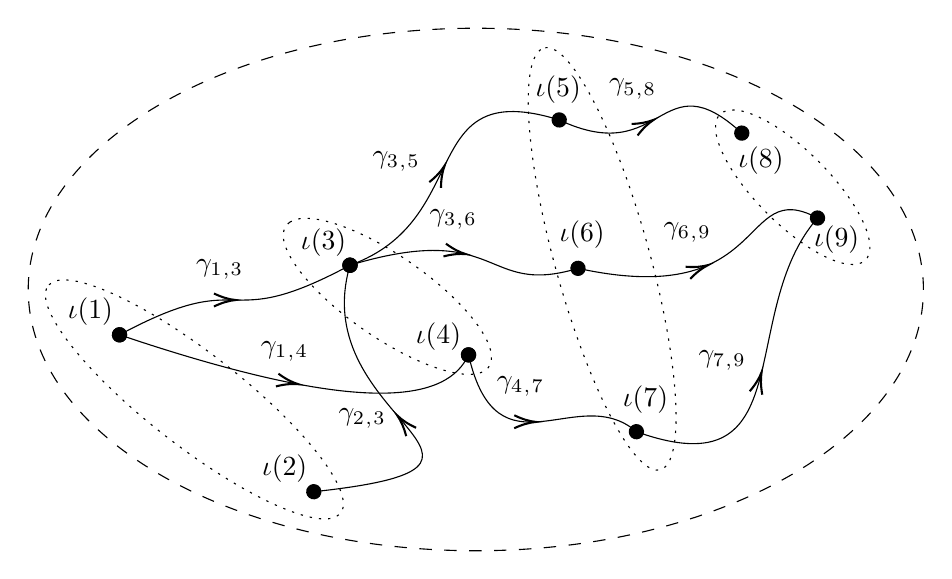
\begin{tikzpicture}[x=0.75pt,y=0.75pt,yscale=-0.95,xscale=0.95]
%uncomment if require: \path (0,281); %set diagram left start at 0, and has height of 281

%Shape: Ellipse [id:dp45216116111361904] 
\draw  [dash pattern={on 4.5pt off 4.5pt}] (6,138.5) .. controls (6,65.32) and (107.63,6) .. (233,6) .. controls (358.37,6) and (460,65.32) .. (460,138.5) .. controls (460,211.68) and (358.37,271) .. (233,271) .. controls (107.63,271) and (6,211.68) .. (6,138.5) -- cycle ;
%Curve Lines [id:da12378300176275903] 
\draw    (52.31,161.49) .. controls (119.1,125.59) and (102.4,162.09) .. (169.19,126.19) ;
\draw [shift={(169.19,126.19)}, rotate = 331.74] [color={rgb, 255:red, 0; green, 0; blue, 0 }  ][fill={rgb, 255:red, 0; green, 0; blue, 0 }  ][line width=0.75]      (0, 0) circle [x radius= 3.35, y radius= 3.35]   ;
\draw [shift={(111.13,143.84)}, rotate = 180.1] [color={rgb, 255:red, 0; green, 0; blue, 0 }  ][line width=0.75]    (10.93,-3.29) .. controls (6.95,-1.4) and (3.31,-0.3) .. (0,0) .. controls (3.31,0.3) and (6.95,1.4) .. (10.93,3.29)   ;
\draw [shift={(52.31,161.49)}, rotate = 331.74] [color={rgb, 255:red, 0; green, 0; blue, 0 }  ][fill={rgb, 255:red, 0; green, 0; blue, 0 }  ][line width=0.75]      (0, 0) circle [x radius= 3.35, y radius= 3.35]   ;
%Curve Lines [id:da3902364739215902] 
\draw    (169.19,126.19) .. controls (233.04,103.33) and (202.45,29.92) .. (275.29,52.51) ;
\draw [shift={(275.29,52.51)}, rotate = 17.23] [color={rgb, 255:red, 0; green, 0; blue, 0 }  ][fill={rgb, 255:red, 0; green, 0; blue, 0 }  ][line width=0.75]      (0, 0) circle [x radius= 3.35, y radius= 3.35]   ;
\draw [shift={(217.18,75.67)}, rotate = 476.11] [color={rgb, 255:red, 0; green, 0; blue, 0 }  ][line width=0.75]    (10.93,-3.29) .. controls (6.95,-1.4) and (3.31,-0.3) .. (0,0) .. controls (3.31,0.3) and (6.95,1.4) .. (10.93,3.29)   ;
\draw [shift={(169.19,126.19)}, rotate = 340.3] [color={rgb, 255:red, 0; green, 0; blue, 0 }  ][fill={rgb, 255:red, 0; green, 0; blue, 0 }  ][line width=0.75]      (0, 0) circle [x radius= 3.35, y radius= 3.35]   ;
%Curve Lines [id:da5125133831866234] 
\draw    (52.31,161.49) .. controls (178.45,204.05) and (218.84,194.46) .. (229.3,171.66) ;
\draw [shift={(229.3,171.66)}, rotate = 294.65] [color={rgb, 255:red, 0; green, 0; blue, 0 }  ][fill={rgb, 255:red, 0; green, 0; blue, 0 }  ][line width=0.75]      (0, 0) circle [x radius= 3.35, y radius= 3.35]   ;
\draw [shift={(142.99,186.54)}, rotate = 191.16] [color={rgb, 255:red, 0; green, 0; blue, 0 }  ][line width=0.75]    (10.93,-3.29) .. controls (6.95,-1.4) and (3.31,-0.3) .. (0,0) .. controls (3.31,0.3) and (6.95,1.4) .. (10.93,3.29)   ;
\draw [shift={(52.31,161.49)}, rotate = 18.65] [color={rgb, 255:red, 0; green, 0; blue, 0 }  ][fill={rgb, 255:red, 0; green, 0; blue, 0 }  ][line width=0.75]      (0, 0) circle [x radius= 3.35, y radius= 3.35]   ;
%Curve Lines [id:da9936282267570157] 
\draw    (150.83,241.06) .. controls (275.76,227.54) and (145.96,205.62) .. (169.19,126.19) ;
\draw [shift={(169.19,126.19)}, rotate = 286.3] [color={rgb, 255:red, 0; green, 0; blue, 0 }  ][fill={rgb, 255:red, 0; green, 0; blue, 0 }  ][line width=0.75]      (0, 0) circle [x radius= 3.35, y radius= 3.35]   ;
\draw [shift={(193.16,202.39)}, rotate = 409.89] [color={rgb, 255:red, 0; green, 0; blue, 0 }  ][line width=0.75]    (10.93,-3.29) .. controls (6.95,-1.4) and (3.31,-0.3) .. (0,0) .. controls (3.31,0.3) and (6.95,1.4) .. (10.93,3.29)   ;
\draw [shift={(150.83,241.06)}, rotate = 353.83] [color={rgb, 255:red, 0; green, 0; blue, 0 }  ][fill={rgb, 255:red, 0; green, 0; blue, 0 }  ][line width=0.75]      (0, 0) circle [x radius= 3.35, y radius= 3.35]   ;
%Curve Lines [id:da37329721640419344] 
\draw    (229.3,171.66) .. controls (243.97,235.64) and (284.76,184.82) .. (314.44,210.62) ;
\draw [shift={(314.44,210.62)}, rotate = 41] [color={rgb, 255:red, 0; green, 0; blue, 0 }  ][fill={rgb, 255:red, 0; green, 0; blue, 0 }  ][line width=0.75]      (0, 0) circle [x radius= 3.35, y radius= 3.35]   ;
\draw [shift={(263.43,205.67)}, rotate = 180.44] [color={rgb, 255:red, 0; green, 0; blue, 0 }  ][line width=0.75]    (10.93,-3.29) .. controls (6.95,-1.4) and (3.31,-0.3) .. (0,0) .. controls (3.31,0.3) and (6.95,1.4) .. (10.93,3.29)   ;
\draw [shift={(229.3,171.66)}, rotate = 77.09] [color={rgb, 255:red, 0; green, 0; blue, 0 }  ][fill={rgb, 255:red, 0; green, 0; blue, 0 }  ][line width=0.75]      (0, 0) circle [x radius= 3.35, y radius= 3.35]   ;
%Curve Lines [id:da6402293447536181] 
\draw    (169.19,126.19) .. controls (246.58,102.99) and (236.29,142.42) .. (284.82,127.77) ;
\draw [shift={(284.82,127.77)}, rotate = 343.19] [color={rgb, 255:red, 0; green, 0; blue, 0 }  ][fill={rgb, 255:red, 0; green, 0; blue, 0 }  ][line width=0.75]      (0, 0) circle [x radius= 3.35, y radius= 3.35]   ;
\draw [shift={(227.95,120.58)}, rotate = 190.98] [color={rgb, 255:red, 0; green, 0; blue, 0 }  ][line width=0.75]    (10.93,-3.29) .. controls (6.95,-1.4) and (3.31,-0.3) .. (0,0) .. controls (3.31,0.3) and (6.95,1.4) .. (10.93,3.29)   ;
%Curve Lines [id:da7275544623824886] 
\draw    (314.44,210.62) .. controls (399.23,240.98) and (364.55,150.12) .. (406.29,102.26) ;
\draw [shift={(406.29,102.26)}, rotate = 311.09] [color={rgb, 255:red, 0; green, 0; blue, 0 }  ][fill={rgb, 255:red, 0; green, 0; blue, 0 }  ][line width=0.75]      (0, 0) circle [x radius= 3.35, y radius= 3.35]   ;
\draw [shift={(377.94,180.41)}, rotate = 465.08] [color={rgb, 255:red, 0; green, 0; blue, 0 }  ][line width=0.75]    (10.93,-3.29) .. controls (6.95,-1.4) and (3.31,-0.3) .. (0,0) .. controls (3.31,0.3) and (6.95,1.4) .. (10.93,3.29)   ;
%Shape: Ellipse [id:dp21247917365246105] 
\draw  [color={rgb, 255:red, 0; green, 0; blue, 0 }  ,draw opacity=1 ][dash pattern={on 0.84pt off 2.51pt}] (16.54,136.11) .. controls (25.63,126.66) and (66.01,145.03) .. (106.72,177.14) .. controls (147.44,209.25) and (173.08,242.94) .. (163.99,252.39) .. controls (154.9,261.85) and (114.52,243.48) .. (73.81,211.37) .. controls (33.09,179.26) and (7.45,145.57) .. (16.54,136.11) -- cycle ;
%Curve Lines [id:da7880732583039812] 
\draw    (275.29,52.51) .. controls (328.72,77.63) and (326.15,20.9) .. (367.89,59.19) ;
\draw [shift={(367.89,59.19)}, rotate = 42.53] [color={rgb, 255:red, 0; green, 0; blue, 0 }  ][fill={rgb, 255:red, 0; green, 0; blue, 0 }  ][line width=0.75]      (0, 0) circle [x radius= 3.35, y radius= 3.35]   ;
\draw [shift={(323.24,52.43)}, rotate = 512.6] [color={rgb, 255:red, 0; green, 0; blue, 0 }  ][line width=0.75]    (10.93,-3.29) .. controls (6.95,-1.4) and (3.31,-0.3) .. (0,0) .. controls (3.31,0.3) and (6.95,1.4) .. (10.93,3.29)   ;
%Curve Lines [id:da726151739669847] 
\draw    (284.82,127.77) .. controls (383.33,149.3) and (366.22,80.72) .. (406.29,102.26) ;
\draw [shift={(350.78,126.12)}, rotate = 518.99] [color={rgb, 255:red, 0; green, 0; blue, 0 }  ][line width=0.75]    (10.93,-3.29) .. controls (6.95,-1.4) and (3.31,-0.3) .. (0,0) .. controls (3.31,0.3) and (6.95,1.4) .. (10.93,3.29)   ;
%Shape: Ellipse [id:dp20693904539608654] 
\draw  [color={rgb, 255:red, 0; green, 0; blue, 0 }  ,draw opacity=1 ][dash pattern={on 0.84pt off 2.51pt}] (138.62,104.37) .. controls (148.74,97.58) and (179.13,108.92) .. (206.48,129.69) .. controls (233.84,150.47) and (247.81,172.81) .. (237.69,179.59) .. controls (227.57,186.38) and (197.19,175.04) .. (169.83,154.27) .. controls (142.47,133.49) and (128.5,111.15) .. (138.62,104.37) -- cycle ;
%Shape: Ellipse [id:dp4442811176180146] 
\draw  [dash pattern={on 0.84pt off 2.51pt}] (268.26,15.88) .. controls (281.5,13.99) and (305.14,60.41) .. (321.05,119.55) .. controls (336.96,178.69) and (339.13,228.17) .. (325.89,230.05) .. controls (312.64,231.94) and (289.01,185.52) .. (273.09,126.38) .. controls (257.18,67.24) and (255.02,17.76) .. (268.26,15.88) -- cycle ;
%Shape: Ellipse [id:dp2537302094398456] 
\draw  [dash pattern={on 0.84pt off 2.51pt}] (358.5,48.46) .. controls (367.96,43.55) and (391.4,56.66) .. (410.84,77.74) .. controls (430.28,98.83) and (438.37,119.9) .. (428.91,124.82) .. controls (419.45,129.73) and (396.01,116.62) .. (376.57,95.54) .. controls (357.13,74.45) and (349.04,53.37) .. (358.5,48.46) -- cycle ;

% Text Node
\draw (50.31,158.09) node [anchor=south east] [inner sep=0.75pt]    {$\iota ( 1)$};
% Text Node
\draw (148.83,237.66) node [anchor=south east] [inner sep=0.75pt]    {$\iota ( 2)$};
% Text Node
\draw (168.57,122.92) node [anchor=south east] [inner sep=0.75pt]    {$\iota ( 3)$};
% Text Node
\draw (226.84,170.66) node [anchor=south east] [inner sep=0.75pt]    {$\iota ( 4)$};
% Text Node
\draw (262.03,45.25) node [anchor=south west] [inner sep=0.75pt]    {$\iota ( 5)$};
% Text Node
\draw (274.13,119.08) node [anchor=south west] [inner sep=0.75pt]    {$\iota ( 6)$};
% Text Node
\draw (306.28,202.6) node [anchor=south west] [inner sep=0.75pt]    {$\iota ( 7)$};
% Text Node
\draw (364.82,65) node [anchor=north west][inner sep=0.75pt]    {$\iota ( 8)$};
% Text Node
\draw (403.23,105) node [anchor=north west][inner sep=0.75pt]    {$\iota ( 9)$};
% Text Node
\draw (89.78,121.75) node [anchor=north west][inner sep=0.75pt]    {$\gamma _{1}{}_{,}{}_{3}$};
% Text Node
\draw (122.67,163.43) node [anchor=north west][inner sep=0.75pt]    {$\gamma _{1}{}_{,}{}_{4}$};
% Text Node
\draw (162.08,197.67) node [anchor=north west][inner sep=0.75pt]    {$\gamma _{2}{}_{,}{}_{3}$};
% Text Node
\draw (179.33,67.29) node [anchor=north west][inner sep=0.75pt]    {$\gamma _{3}{}_{,}{}_{5}$};
% Text Node
\draw (208.3,96.52) node [anchor=north west][inner sep=0.75pt]    {$\gamma _{3}{}_{,}{}_{6}$};
% Text Node
\draw (242.33,181.1) node [anchor=north west][inner sep=0.75pt]    {$\gamma _{4}{}_{,}{}_{7}$};
% Text Node
\draw (299.22,30.41) node [anchor=north west][inner sep=0.75pt]    {$\gamma _{5}{}_{,}{}_{8}$};
% Text Node
\draw (326.9,103.09) node [anchor=north west][inner sep=0.75pt]    {$\gamma _{6}{}_{,}{}_{9}$};
% Text Node
\draw (344.63,168.21) node [anchor=north west][inner sep=0.75pt]    {$\gamma _{7}{}_{,}{}_{9}$};


\end{tikzpicture}


\end{center}
\caption{A Transport Graph in a Surface}
\end{figure}
Notice that we can describe this transport graph with an ``algebraic''
expression of the form:
\[
  (\gamma_{5, 8} \tensor (\gamma_{6, 9} \cdot \gamma_{7, 9})) \circ
  (\gamma_{3, 5} \tensor \gamma_{3, 6} \tensor \gamma_{4, 7}) \circ
  ((\gamma_{1, 3} \cdot \gamma_{2, 3}) \tensor \gamma_{1, 4})
\]
where the rule of forming such an expression is roughly to connect
expressions between two consecutive parts with the ``same end point'' with a
`$\cdot$', expressions between two consecutive parts without the
``same end-point'' with a `$\tensor$' and ``composeable'' expressions with a
`$\circ$'. We note that if end-points are replaces with copies of an algebra $A$
and paths, with appropriate linear maps, the whole expression is also a linear
map from some tensor power of $A$ to another tensor power of $A$.
\end{exm}

We observe that we can take disjoint unions of manifolds equipped with transport
graphs but the result is not a transport graph in general. For this, we define
the following.

\begin{defn}[Transport Forest (First Attempt)]
A disjoint union of transport graphs $G = G_1 \amalg \dots \amalg G_n$ is called
a transport forest. We have a part function for each component transport graph --
that is, $p_{G_i}(u) = j$ if and only if $u \in G_i$, the vertex set of $G_i$ is
$V_{i, 1} \amalg \dots \amalg V_{i, k}$ and $u \in V_{i, j}$.
\end{defn}

It is then easy to see that taking the disjoint union of two manifolds $M$ and
$N$ equipped with transport forests $G$ and $H$ respectively along with the
disjoint union of $G$ and $H$, yields a manifold $M \amalg N$ with a transport
forest $G \amalg H$ in $M \amalg N$. In particular, we can consider the empty
manifold equipped with the empty forest as a zero-fold disjoint union of
transport forests in manifolds. Associators and unitors from the category of
sets then yield associators and unitors for transport forests. In order to
obtain a monoidal category of transport forests, we define the following notion.

\begin{defn}[Transport Homomorphism (First Attempt)]
Let
\[
  G = \coprod_{i = 1}^{n} G_i = ((V_G, E_G), \iota_G, \gamma^G_{-, -})
  \text{ and }
  H = \coprod_{j = 1}^{m} H_j = ((V_H, E_H), \iota_H, \gamma^H_{-, -})
\]
be transport forests in manifolds $M$ and $N$ respectively. Then, a
graph homomorphism $h : (V_G, E_G) \to (V_H, E_H)$ satisfying
\begin{enumerate}[(i)]
\item for all $i \in \set{1, \dots, n}$, $h(G_i) \subset H_j$ for some
$j \in \set{1, \dots, m}$
\item $p_{G_i}(u) = p_{G_i}(v) \iff p_{H_j}(h(u)) = p_{H_j}(h(v))$
\end{enumerate}
along with a smooth map $f : M \to N$ making the following diagrams commute is
called a morphism of transport forests in manifolds or a transport homomorphism:
\[
\begin{tikzpicture}[baseline=(a).base]
\node[scale=\diagscale] (a) at (0, 0){
\begin{tikzcd}
E_G \ar[d, "\gamma^G_{-, -}" left] \ar[r, "h" above] &
E_H \ar[d, "\gamma^H_{-, -}" right] \\
C^0(I, M) \ar[r, "f_*" below] &
C^0(I, N)
\end{tikzcd}
};
\end{tikzpicture}
\]
where $f_*$ is the post-composition map $g \mapsto f \circ g$.
\end{defn}

\begin{rmk}
The condition in the above definition ensures that $h$ restricted to each
transport graph in its domain forest is also a homomorphism into a transport
graph in the codomain forest. It also ensures that the images of $h$ and $f^*$
together form a transport forest.
\end{rmk}

Pasting the commutative squares as the above along the $\gamma$ sides, we observe
that morphisms of transport forests in manifolds compose associatively. Taking
$h$ and $f$ as the identity maps yields an identity morphism of transport
forests. This yields the following theorem.

\begin{thm}
Transport forests in manifolds along with transport homomorphisms form a monoidal
category with disjoint union as the monoidal product and the empty manifolds
equipped with the empty transport forests as monoidal units.
\end{thm}

\begin{defn}
The monoidal category of the above theorem is called the category of transport
forests in manifolds and denoted $\TF$. The monoidal subcategory of $\TF$
consisting on manifolds of a fixed dimension $d$ is denoted $\TF_d$.
\end{defn}

\subsection{Connections with Transport Forests}

We have a notion of gluing for cobordisms of a fixed dimension that gives
$\Cob_d$ the structure of a monoidal bicategory. We now try to extend this to
connections and transport forests. This will yield a bicategory that will
function as the domain of our notion of TQFTs which can handle quantum
information.

We first address the notion of gluing transport forests. We define the ``source''
and ``target'' ends of a transport forest in the obvious way.
\begin{defn}
Let $G = \coprod_{i = 1}^{n} G_i$ be a transport graph on a manifold $M$ with
$G_i$ having the vertex partition $\coprod_{j = 1}^{k_i} V_{i, j}$. Then, we
define the source of $G$ as $S(G) = \coprod_{i = 1}^{n} V_{i, 1}$ and the target
of $G$ as $T(G) = \coprod_{i = 1}^{n} V_{i, k_i}$.
\end{defn}

\begin{rmk}
We notice that the total ordering of vertex set parts of each transport graph in
a transport forest along with the ordering of the transport graphs themselves in
the transport induces a total ordering of $S(G)$ and $T(G)$ respectively.
\end{rmk}

\begin{defn}
Let $G$ and $H$ be transport forests in manifolds $M$ and $N$ respectively such
that $|S(H)| = |T(G)|$. Let $X \to[a_M] M \ot[b_M] Y$ and
$Y \to[a_N] N \ot[b_N] Z$ be cobordisms of some dimension $d$. We then have
$S(H)$ and $T(G)$ totally ordered with a unique order-preserving bijection
$\psi_{G, H} : T(G) \to S(H)$. Then, we define a gluing operation in $\TF_d$ as
follows:
\[
  (N, H) * (M, G) = (M \amalg_{Y} N, G \amalg_{T(G)} H)
\]
where the gluing $\amalg_{T(G)}$ is the pushout of the diagram
$G \hookleftarrow T(G) \stackrel{\psi_{G, H}}{\hookrightarrow} H$ in
$\Set$.
\end{defn}

We now wish to define a unit for this gluing operation. Given a cobordism
$X \to M \ot Y$ with a transport forest $G$ in $M$, the gluing identities of $M$
in $\Cob_d$ are the cylinder $X \times I$ and $Y \times I$ on $Y$. Then, the
gluing identities of $G$ should be a transport forests in $X \times I$ and
$Y \times I$ that act like cylinders on $S(G)$ and $T(G)$ respectively. For
simplicity, we consider that this ``cylinder'' on $S(G)$ is the graph with
vertex set $V = V_1 \amalg V_2$ where each $V_i$ is isomorphic to $S(G)$ with an
order preserving isomorphism. The edges are $(u, v)$ where $u \in V_1$ and
$v \in V_2$ are in the same order position. Then $\gamma_{u, v}$ is some path
in $X \times I$ which will hopefully yield the identity linear map under
parallel transport with respect to some connection. We call this graph
$1_{S(G)}$. Such a graph on a surface could look like the following, for
instance:
\begin{figure}[H]
\begin{center}

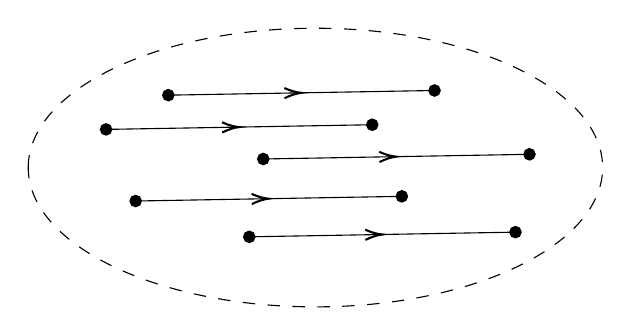
\begin{tikzpicture}[x=0.75pt,y=0.75pt,yscale=-0.75,xscale=0.75]
%uncomment if require: \path (0,300); %set diagram left start at 0, and has height of 300

%Straight Lines [id:da5492592026359605]
\draw    (200,94) -- (371,91) ;
\draw [shift={(371,91)}, rotate = 358.99] [color={rgb, 255:red, 0; green, 0; blue, 0 }  ][fill={rgb, 255:red, 0; green, 0; blue, 0 }  ][line width=0.75]      (0, 0) circle [x radius= 3.35, y radius= 3.35]   ;
\draw [shift={(285.5,92.5)}, rotate = 538.99] [color={rgb, 255:red, 0; green, 0; blue, 0 }  ][line width=0.75]    (10.93,-3.29) .. controls (6.95,-1.4) and (3.31,-0.3) .. (0,0) .. controls (3.31,0.3) and (6.95,1.4) .. (10.93,3.29)   ;
\draw [shift={(200,94)}, rotate = 358.99] [color={rgb, 255:red, 0; green, 0; blue, 0 }  ][fill={rgb, 255:red, 0; green, 0; blue, 0 }  ][line width=0.75]      (0, 0) circle [x radius= 3.35, y radius= 3.35]   ;
%Straight Lines [id:da20474186640834924]
\draw    (160,116) -- (331,113) ;
\draw [shift={(331,113)}, rotate = 358.99] [color={rgb, 255:red, 0; green, 0; blue, 0 }  ][fill={rgb, 255:red, 0; green, 0; blue, 0 }  ][line width=0.75]      (0, 0) circle [x radius= 3.35, y radius= 3.35]   ;
\draw [shift={(245.5,114.5)}, rotate = 538.99] [color={rgb, 255:red, 0; green, 0; blue, 0 }  ][line width=0.75]    (10.93,-3.29) .. controls (6.95,-1.4) and (3.31,-0.3) .. (0,0) .. controls (3.31,0.3) and (6.95,1.4) .. (10.93,3.29)   ;
\draw [shift={(160,116)}, rotate = 358.99] [color={rgb, 255:red, 0; green, 0; blue, 0 }  ][fill={rgb, 255:red, 0; green, 0; blue, 0 }  ][line width=0.75]      (0, 0) circle [x radius= 3.35, y radius= 3.35]   ;
%Straight Lines [id:da4667779836114062]
\draw    (252,185) -- (423,182) ;
\draw [shift={(423,182)}, rotate = 358.99] [color={rgb, 255:red, 0; green, 0; blue, 0 }  ][fill={rgb, 255:red, 0; green, 0; blue, 0 }  ][line width=0.75]      (0, 0) circle [x radius= 3.35, y radius= 3.35]   ;
\draw [shift={(337.5,183.5)}, rotate = 538.99] [color={rgb, 255:red, 0; green, 0; blue, 0 }  ][line width=0.75]    (10.93,-3.29) .. controls (6.95,-1.4) and (3.31,-0.3) .. (0,0) .. controls (3.31,0.3) and (6.95,1.4) .. (10.93,3.29)   ;
\draw [shift={(252,185)}, rotate = 358.99] [color={rgb, 255:red, 0; green, 0; blue, 0 }  ][fill={rgb, 255:red, 0; green, 0; blue, 0 }  ][line width=0.75]      (0, 0) circle [x radius= 3.35, y radius= 3.35]   ;
%Straight Lines [id:da4241115453701192]
\draw    (261,135) -- (432,132) ;
\draw [shift={(432,132)}, rotate = 358.99] [color={rgb, 255:red, 0; green, 0; blue, 0 }  ][fill={rgb, 255:red, 0; green, 0; blue, 0 }  ][line width=0.75]      (0, 0) circle [x radius= 3.35, y radius= 3.35]   ;
\draw [shift={(346.5,133.5)}, rotate = 538.99] [color={rgb, 255:red, 0; green, 0; blue, 0 }  ][line width=0.75]    (10.93,-3.29) .. controls (6.95,-1.4) and (3.31,-0.3) .. (0,0) .. controls (3.31,0.3) and (6.95,1.4) .. (10.93,3.29)   ;
\draw [shift={(261,135)}, rotate = 358.99] [color={rgb, 255:red, 0; green, 0; blue, 0 }  ][fill={rgb, 255:red, 0; green, 0; blue, 0 }  ][line width=0.75]      (0, 0) circle [x radius= 3.35, y radius= 3.35]   ;
%Straight Lines [id:da7354211412427432]
\draw    (179,162) -- (350,159) ;
\draw [shift={(350,159)}, rotate = 358.99] [color={rgb, 255:red, 0; green, 0; blue, 0 }  ][fill={rgb, 255:red, 0; green, 0; blue, 0 }  ][line width=0.75]      (0, 0) circle [x radius= 3.35, y radius= 3.35]   ;
\draw [shift={(264.5,160.5)}, rotate = 538.99] [color={rgb, 255:red, 0; green, 0; blue, 0 }  ][line width=0.75]    (10.93,-3.29) .. controls (6.95,-1.4) and (3.31,-0.3) .. (0,0) .. controls (3.31,0.3) and (6.95,1.4) .. (10.93,3.29)   ;
\draw [shift={(179,162)}, rotate = 358.99] [color={rgb, 255:red, 0; green, 0; blue, 0 }  ][fill={rgb, 255:red, 0; green, 0; blue, 0 }  ][line width=0.75]      (0, 0) circle [x radius= 3.35, y radius= 3.35]   ;
%Shape: Ellipse [id:dp23218831414777463]
\draw  [dash pattern={on 4.5pt off 4.5pt}] (110,140.5) .. controls (110,91.07) and (192.6,51) .. (294.5,51) .. controls (396.4,51) and (479,91.07) .. (479,140.5) .. controls (479,189.93) and (396.4,230) .. (294.5,230) .. controls (192.6,230) and (110,189.93) .. (110,140.5) -- cycle ;

\end{tikzpicture}


\end{center}
\caption{A ``Cylinder'' Transport Forest}
\end{figure}

The issue, however, is that there is no transport homomorphism
\[
  ((X \times I) \amalg_X M, 1_{S(G)} \amalg_{S(G)} G) \to (M, G)
\]
because $1_{S(G)}$ cannot be collapsed to $S(G)$ as $S(G)$ has no self edges.
There is no transport homomorphism in the other direction either because we
cannot ``expand'' $S(G)$ to $1_{S(G)}$ since this would require the duplication
of vertices and creation of edges from none. We are thus forced to modify our
definition of transport forests and transport homomorphisms. In particular, we
add self-loops in transport graphs and forests. We start redefining these
notions as follows, with modifications in bold.

\begin{defn}[Transport Graph]
Let $G = (V, E)$ be a finite directed graph satisfying the following properties:
\begin{enumerate}[(i)]
\setlength{\itemsep}{0pt}
\item $V = V_1 \amalg \dots \amalg V_k$ for some $k \geq 2 \in \N$, with each
$V_i$ totally ordered as $V_i = \set{v_{i, 1}, \dots, v_{i, q_i}}$ for some
$q_i \in \N$
\item each point in $V_{i + 1}$ has at least one edge from a point in $V_{i}$,
$1 \leq i < k$
\item each point in $V_{i}$ has at least one edge to a point in $V_{i + 1}$,
$1 \leq i < k$
\item \textbf{for every vertex $u$, there exists exactly one loop $(u, u) \in E$
on $u$}
\item if $(u, v) \in E$, then \textbf{either $u = v$ or} $u \in V_i$ and
$v \in V_{i + 1}$ for some $i \in \set{1, \dots, k - 1}$
\end{enumerate}
Then $G$ is called a transport graph and for any vertex $v \in V$, we write
$p_{G}(v)$ to denote the part of which $v$ is an element -- that is,
$p_G(v) = i$ if and only if $v \in V_i$.
\end{defn}

%\begin{defn}[Admissible Transport Graph in a Manifold]
%We call a transport graph in a manifold admissible if $\gamma_{u, u}$ is the
%constant path on some point.
%\end{defn}

\begin{defn}[Graph Multimorphism]
Let $G = (V, E)$ and $H = (V', E')$ be directed graphs. Let $f : V \to V'$ be a
relation such that for every $u \in V$, there exists $v' \in V'$ with
$(v, v') \in f$ every pair of vertices $u, v \in V$ and for every
$(u, u'), (v, v') \in f$, if $(u, v)$ is an edge in $G$ then $(u', v')$ is an
edge in $H$. Then, $f$ is called a graph multimorphism.\footnote{We note that
this definition is identical to the one given in \cite{PcLinTop}. Although we
defined this before consulting \cite{PcLinTop}, the definition there reminded us
that a relation need not have an image for every point in the domain.
\textbf{This footnote is mainly for Steve. We may remove most of it in the
final write-up.}}
\end{defn}

\begin{defn}
The relational composites of graph multimorphisms are again graph
multimorphisms so that directed graphs with multimorphisms form a category. We
denote this category $\DGraph_{\Rel}$.
\end{defn}

\begin{defn}[Transport Homomorphism]
Let
\[
  G = \coprod_{i = 1}^{n} G_i = ((V_G, E_G), \iota_G, \gamma^G_{-, -})
  \text{ and }
  H = \coprod_{j = 1}^{m} H_j = ((V_H, E_H), \iota_H, \gamma^H_{-, -})
\]
be transport forests in manifolds $M$ and $N$ respectively. Then, a graph
\textbf{multimorphism} $h : (V_G, E_G) \to (V_H, E_H)$ satisfying
\begin{enumerate}[(i)]
\item for all $i \in \set{1, \dots, n}$, $h(G_i) \subset H_j$ for some
$j \in \set{1, \dots, m}$
\item $p_{G_i}(u) = p_{G_i}(v) \iff p_{H_j}(h(u)) = p_{H_j}(h(v))$
\end{enumerate}
along with a smooth map $f : M \to N$ making the following diagram commute
\textbf{in $\Rel$} is called a morphism of transport forests in manifolds or a
transport homomorphism:
\[
\begin{tikzpicture}[baseline=(a).base]
\node[scale=\diagscale] (a) at (0, 0){
\begin{tikzcd}
E_G \ar[d, "\gamma^G_{-, -}" left] \ar[r, "h" above] &
E_H \ar[d, "\gamma^H_{-, -}" right] \\
C^0(I, M) \ar[r, "f_*" below] &
C^0(I, N)
\end{tikzcd}
};
\end{tikzpicture}
\]
where $f_*$ is the post-composition map $g \mapsto f \circ g$.
\end{defn}

It is now easy to see that there is a transport homomorphism, in this new sense,
\[
  \phi : ((X \times I) \amalg_X M, 1_{S(G)} \amalg_{S(G)} G) \longleftrightarrow
         (M, G) : \psi
\]
defined in the obvious way by ``collapsing'' $1_{S(G)}$ to $S(G)$ by sending the
edges, including loops, in $1_{S(G)}$ to the corresponding loops in $S(G)$; and,
for the other direction, ``exapanding'' $S(G)$ to $1_{S(G)}$ by ``duplicating''
loops on $S(G)$ into corresponding edges and loops in $1_{S(G)}$, respectively.

\TODO{This collapsing of edges and expanding of vertices might have issues at
the very end of paths in diffeomorphism groups. For instance, for all but one of
the points in the path from $\id$ to $\phi$ in the diffeomorphism group, the
associated graph multimorphism is the identity but suddenly, at the end point,
it is a collapse of several edges. We might need a truly geometric formulation
of trasport graphs that still remembers the graph theoretic data -- I think the
graph theoretic data is essential. There may, however, be hope in the fact that
the graph theoretic data has essentially nothing to do with the smooth data --
more on this in a possible meeting, perhaps.}

\end{document}

